\documentclass[a4paper]{article}

%% Language and font encodings
\usepackage[english]{babel}
\usepackage[utf8x]{inputenc}
\usepackage[T1]{fontenc}

%% Sets page size and margins
\usepackage[a4paper,top=3cm,bottom=2cm,left=3cm,right=3cm,marginparwidth=1.75cm]{geometry}

%% Useful packages
\usepackage{amsmath}
\usepackage{graphicx}
\usepackage[colorinlistoftodos]{todonotes}
\usepackage[colorlinks=true, allcolors=blue]{hyperref}
\usepackage{wrapfig}

\usepackage{tikz} %Tikz !
\usetikzlibrary{arrows,automata,calc}

\hypersetup{
	urlcolor= blue,  %couleur des hyperliens
	linkcolor= black, %couleur des liens internes
}


\newcommand{\HRule}{\rule{\linewidth}{0.5mm}} % Defines a new command for the horizontal lines, change thickness here



\title{Robotique en essaim}
\author{Andres Julien, Taylor Thomas}
\date{}
\begin{document}

\begin{titlepage}
\center
\includegraphics{/home/julien/Images/LOGO_SCIENCES_SU_med.jpg}\\[1cm] 

\HRule \\[0.4cm]
{ \huge \bfseries Robotique en essaim}\\[0.4cm] % Title of your document
\HRule \\[1.5cm]



Julien \textsc{Andres}\\ % Your name
Thomas \textsc{Taylor}\\[3cm]
Nicolas \textsc{Bredeche}\\[3cm]


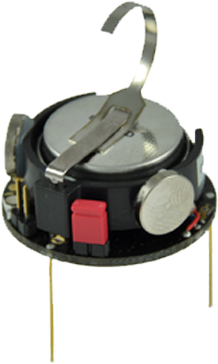
\includegraphics[width=4cm]{/home/julien/Images/Kilobots.png}



\end{titlepage}

\newpage
\renewcommand{\contentsname}{Sommaire}
\tableofcontents
\newpage
\section{Introduction}
\subsection{Robotique en essaim}
La robotique en essaim s'inspire d'observations d'insectes et d'animaux sociaux pour l'étude de comportements collectifs issus de simples tâches individuelles. Les principales propriétés de ce domaine sont la robustesse, grâce à un code décentralisé, et l'échelle proposée, le code pouvant être déployé sur différentes tailles d'essaim.
\subsection{Couverture}
La couverture est un problème fondamental dans la robotique en essaim. En effet, elle permet aux robots de se déployer dans un environnement inconnu ou dynamiques, tout en maintenant un contact entre eux. Ce problème se retrouve dans beaucoup de domaine, comme le sauvetage de personnes en milieu hostile ou inconnu.
\subsection{Agrégation}
L'agrégation est un comportement de base des essaims. Il permet aux organismes de faire face ensemble à un problème. Dans le domaine de la robotique en essaim, ce comportement permet a des robots dispersés dans un environnement de se regrouper en un ou plusieurs groupes.
\subsection{Algorithmes génétiques en ligne}
L'objectif de ces algorithmes est d'arriver, à partir d'un génome aléatoire définissant un comportement d'un robot, à un comportement permettant au robot de survivre dans son environnement. L'aspect \textit{en-ligne} de l'algorithme représente la distribution du code sur l'ensemble des robots. ??? ajouter apprentissage ensemble ??
\subsection{Problématique}
\newpage
\section{Matériel utilisé}
\subsection{Kilobot}
Un Kilobot est un robot miniature, créé par l'université d'Harvard. Ces robots permettent l'étude de la robotique en essaim grâce à leur faible cout, permettant grand nombre d'individu.
\paragraph{Communication}Les robots peuvent communiquer entre eux grâce à des messages qu'ils envoient à leurs voisins à une distance d'environ 7cm. L'intensité du signal permet à un Kilobot d'évaluer la distance à laquelle se trouve la source du message. Chaque robot possède aussi un capteur de luminosité.
\paragraph{Mouvements}Chaque robot possède deux moteurs, placé de chaque coté de son corps. Ils permettent au robot d'avancer en faisant vibrer ses pattes. Les déplacement d'un Kilobot se font donc en modulant la vitesse de chacun de ses moteurs selon la direction voulu.\\
\begin{figure}[h]
	\begin{center}
		\centering
		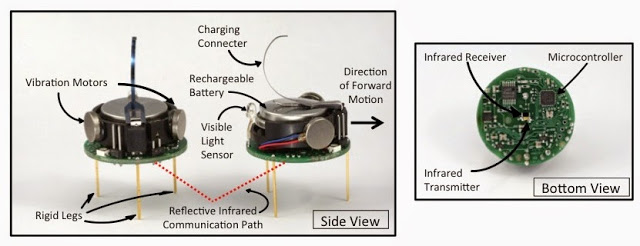
\includegraphics[width=0.8\linewidth]{kilobot-closeup-overview.jpg}
		\caption{Kilobot}
	\end{center}
\end{figure} \\
Les comportements des robots sont écrits en C, en utilisant l'API kilolib et peut être transmis à l'ensemble des Kilobots  grâce à un contrôleur infrarouge.
reçoit
\subsection{Bloc Actif}
Le bloc actif a été développé par l'ISIR dans le cadre de la recherche sur Kilobots. Elle permet d'interagir avec les robots en émettant un signal infrarouge. Le numéro du message et l'intensité du signal peuvent être modulé grâce à des boutons sur le bloc actif. Il fera office d'obstacle et de point de ralliement pour certains de nos algorithmes.\\
PHOTO BLOC ACTIF intensité Max et min
\subsection{Arène}
Les algorithmes ont été testé sur un essaim de 70 robots, fournit par le laboratoire de rechercher ISIR. L'arène utilisé pour l'étude des algorithme faisait 1x2 mètres.\\
PHOTO ARENE
\subsection{Simulateur}
Afin de faciliter le développement et l'étude des algorithmes, le simulateur Kilombo a été utilisé. Il inclut l'API kilolib et permet ainsi une compatibilité direct du code entre le simulateur et l'essaim de robots.
SCREENSHOT ?
\newpage
\section{Couverture}
\subsection{Algorithme}
Cet algorithme est utilisé afin de couvrir la plus grande surface possible, tout en gardant un lien de communication entre les Kilobots.
Il est composé de 3 comportements basique : L'éloignement (\textit{repel}), le déplacement aléatoire(\textit{searching}) et l'attente(\textit{wait})
\paragraph{Le déplacement aléatoire} Ce comportement s'effectue lorsque le Kilobot ne détecte aucun voisin. Il bouge alors aléatoirement dans son environnement jusqu'à la détection d'un autre robot. Il passe alors en mode d'attente ou d'éloignement selon la distance à laquelle il est de ses voisins.
\paragraph{L'éloignement} Si le Kilobot se trouve trop proche de ses voisins, il essayera de s'en éloigner. Soit en s'éloignant de son voisin le plus proche, soit en bougeant aléatoirement jusqu'à être à une distance désiré de tous ses voisins.
\paragraph{L'attente} Le Kilobot entre en attente quand il se trouve à une distance supérieure ou égale à celle demandé de tous ses voisins. Il sort de ce comportement s'il ne capte plus aucun voisins ou si un Kilobot arrive trop proche.\\


\begin{figure}[h!]
\centering
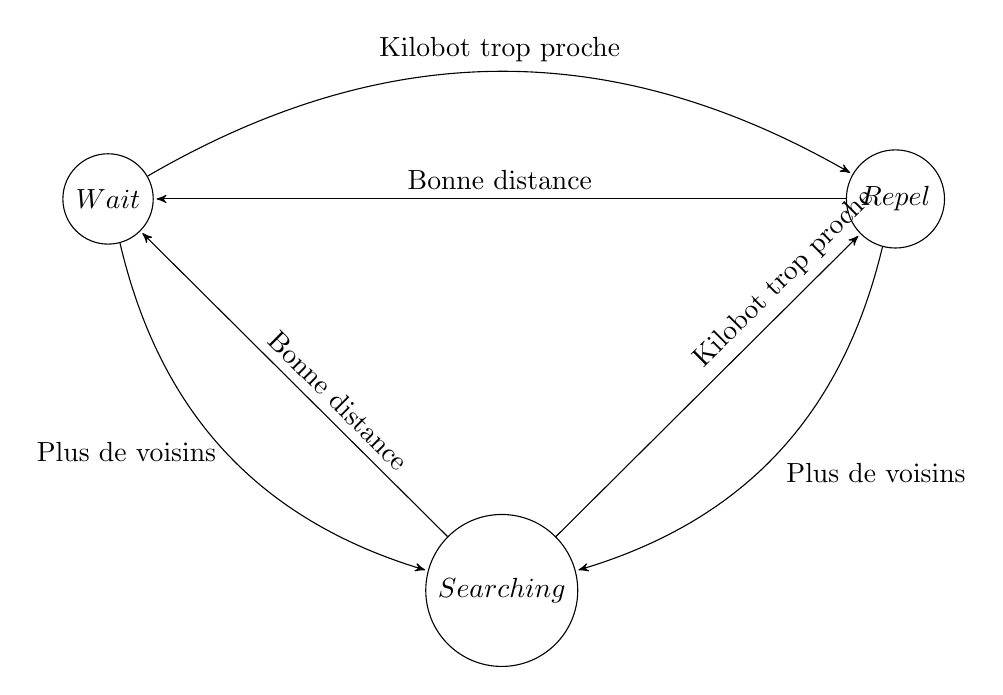
\begin{tikzpicture}[>=stealth',shorten >=1pt,auto,node distance=10cm]
\node[state] (W)      {$Wait$};
\node[state] (R) [right of=W]  {$Repel$};
\node[state] at ($(W)!0.5!(R)$) [below =4cm] (S)  {$Searching$};


\path[->]
(W) edge  [bend left,sloped] node {Kilobot trop proche} (R)
(R) edge   [sloped]node {Bonne distance} (W)
(W) edge   [bend right,anchor=east]node {Plus de voisins} (S)
(S) edge   [sloped,pos=0.4,align=right,anchor=south]node {Bonne distance} (W)
(R) edge   [bend left]node {Plus de voisins} (S)
(S) edge   [sloped,pos=0.8]node {Kilobot trop proche} (R);
\end{tikzpicture}
\caption{Couverture}
\end{figure}

\subsection{Résultats}
\newpage
\section{Agrégation}
\subsection{Agrégation naïve}
\subsection{Agrégation probabiliste}

Cet algorithme découle de celui présenté par O.Soysal et E.Sahin. Il permet aux robots de s'agglomérer basé sur une probabilité calculé indépendamment par chaque robot.\\

Il est composé de 4 comportement basiques : l'approche(\textit{approach}), l'attente(\textit{wait}), l'éloignement (\textit{repel}) et un évitement d'obstacle.
Un Kilobot n'ayant pas de capteur de proximité, il lui est impossible de détecter un obstacle tel qu'un mur. L'évitement d'obstacle a donc été remplacé par un déplacement aléatoire dans l'environnement (\textit{searching}).
\paragraph{Le déplacement aléatoire} Quand le robot est seul dans l'environnement (aucun voisins), il bouge de façon aléatoire. Toute les secondes, il choisi une direction parmi les 3 disponibles (gauche, droite,tout droit) et la garde jusqu'à la prochaine actualisation. Dés qu'il détecte un voisin, il passe en comportement d'approche
\paragraph{L'approche}Dans ce comportement, le robot décide de s'approcher du voisin le plus intéressant. Le voisin le plus intéressant est défini comme le celui ayant le plus de voisins à coté de lui. Si le Kilobot arrive à rejoindre le groupe, ce qui n'est pas obligatoire, à cause de l'absence de capteurs de proximités, il s'arrête et passe dans l'état d'attente.
\paragraph{L'attente} Quand le robot est dans cet état, il fait partit d'un groupe composé d'au moins 2 individus. Il a cependant une probabilité de quitter ce groupe et d'entrer dans l'état d'éloignement à chaque seconde.
\paragraph{L'éloignement}Ce comportement fait s'éloigner le robot du groupe auquel il était agrégé précédemment. Pendant toute la durée de cet éloignement, à chaque seconde, le Kilobot à une probabilité de revenir en mode d'approche et de rejoindre le groupe qu'il vient de quitter. Ce comportement s'arrête quand le robot est seul ou que 10 secondes se sont écoulées. Il revient en déplacement aléatoire.\\
\begin{figure}[h!]
	\centering
	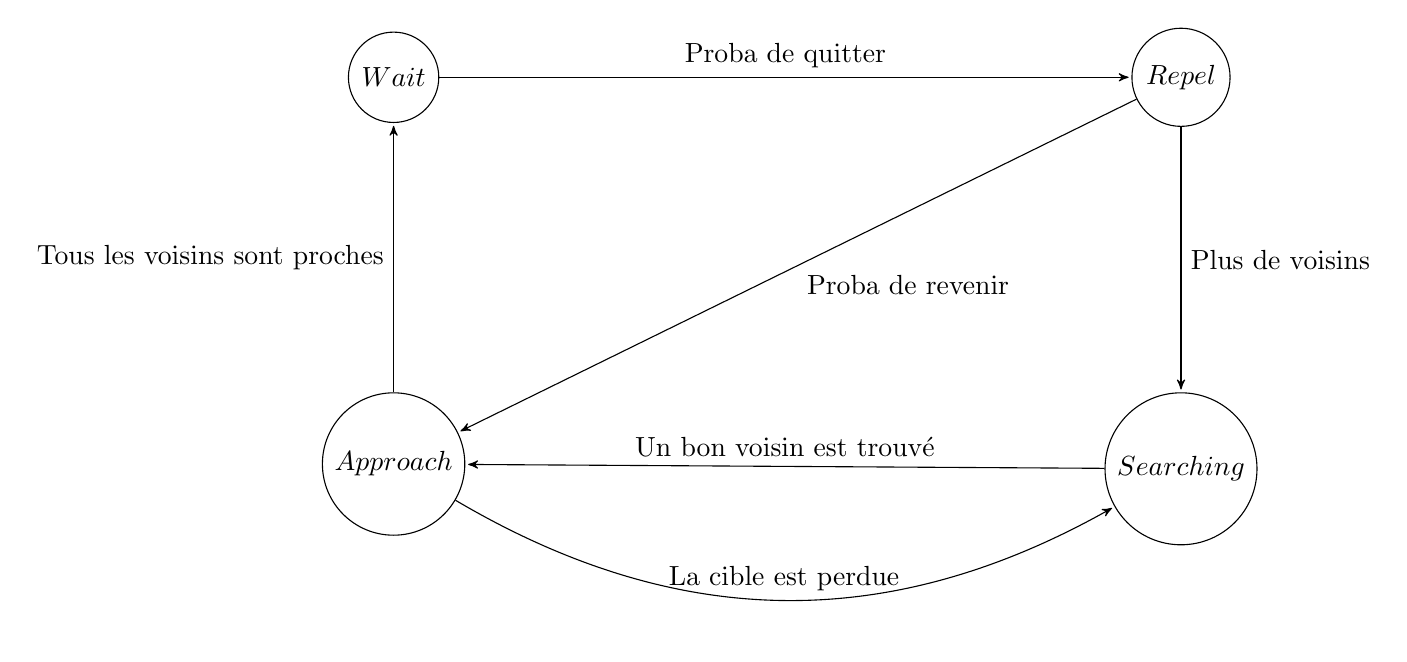
\begin{tikzpicture}[>=stealth',shorten >=1pt,auto,node distance=10cm]
	\node[state] (W)      {$Wait$};
	\node[state] (R) [right of=W]  {$Repel$};
	\node[state] [right of=W,below =4cm] (S)  {$Searching$};
	\node[state] (A)  [below=4cm]{$Approach$};
	
	
	\path[->]
	(A) edge node {Tous les voisins sont proches}(W)
	(S) edge [anchor=south]node {Un bon voisin est trouvé}(A)
	(A) edge [bend right]node {La cible est perdue} (S)
	(W) edge  [sloped] node {Proba de quitter} (R)
	(R) edge   node {Plus de voisins} (S)
	(R) edge node {Proba de revenir} (A)
	;
	\end{tikzpicture}
	\caption{Agrégation probabiliste}
\end{figure}
\newpage
\section{mEDEA}
\subsection{Algorithme}
\subsection{Résultats}
\newpage
\section{Conclusion}
\section{Bibliographie}
\end{document}